\section{Ganzzahlig-lineare Programmierung \skript{63}}
  \begin{minipage}{7cm}
    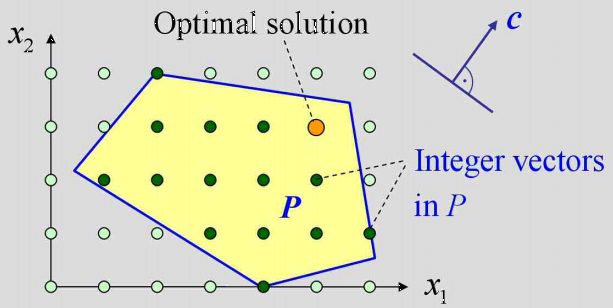
\includegraphics[width=7cm]{./Content/IntProg/intprog}
  \end{minipage}
  \begin{minipage}{12cm}
	  Als zusätzliche Nebenbedingung zu LP dürfen Variablen nur ganzzahlig (integer, ILP) sein, das macht das Problem einiges komplizierter.
	  Konkret sind LP polynomial lösbar, während ILP NP-vollständig (NP-complete) sind.
	    
  	\subsection{Relaxationen}
  		Um Schranken (obere/untere) zu berechnen, kann der \em Lösungsraum
  		vergrössert \em werden (Relaxationen). Beispiel: Der höchste Berg in
  		Tibet ist höchstens so gross wie der höchste Berg in China (China
  		$\rightarrow$ grösserer Lösungsraum als Tibet). In ILP wird \em
  		LP-Relaxation \em verwendet, d.h. die Ganzzahligkeitsforderung wird
  		fallen gelassen.
	\end{minipage}
  
		

\subsection{Branch-and-Bound Verfahren \skript{68}}
	\begin{minipage}{8cm}
		Um die optimale Lösung zu finden, wird das Lösungsgebiet aufgeteilt und jeweils sowohl eine obere als auch eine untere Schranke der Lösung gesucht. Falls die Schranken bereits eine optimale Lösung ausschliessen (wenn bei einem anderen Ast die untere Schranke höher ist als die obere beim aktuellen), kann die Suche innerhalb dieses Astes abgebrochen werden. Man spricht von \em Pruning by Dominance\em. Optimalität ist gefunden, wenn die obere gleich der unteren Schranke ist.
		
		Details für ILP: \skript{72f.}
	\end{minipage}
	\begin{minipage}{10cm}
		Beispiel: Helikopter $\Leftrightarrow$ Sherpas.
		
		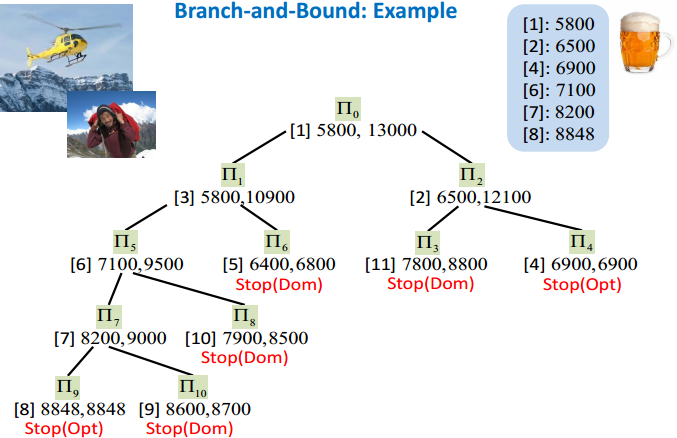
\includegraphics[width=10cm]{Content/IntProg/branch-bound}
	\end{minipage}
  
\subsection{Schnittebenenverfahren (Cutting Planes) \skript{78}}  
	\todo{RK: Keine Übungen dazu gefunden... ZF nötig??}
	
	Durch Linearkombination der Bedingungen, ist eine Einschränkung des Lösungsgebiets möglich. Die Multiplikatoren werden durch "pröbeln" gefunden. Beispiel:
	
	\begin{tabular}{p{8cm} p{4cm} p{3cm}}
		Ursprüngliche Bedingung 1 & $x_1 + 3 x_2 \leq 6$ & $| \cdot \frac{5}{8}$\\
		Ursprüngliche Bedingung 2 & $3 x_1 + x_2 \leq 6$ & $| \cdot \frac{1}{8}$  \\
		Aufsummiert: & $x_1 + 2 x_2 \leq \lfloor 4.5 \rfloor \overbrace{=}^{!} 4$ \\
	\end{tabular}